\documentclass[polish,12pt]{aghthesis}
\usepackage[utf8x]{inputenc}
\usepackage{url}
\usepackage{graphicx}

\graphicspath{ {./images/} }

\author{Piotr Szczygieł}

\titlePL{Gra typu Capture-The-Flag\\ oparta o reverse engineering}
\titleEN{Capture-The-Flag game based on reverse engineering}

\fieldofstudy{Informatyka}

\supervisor{dr inż.\ Łukasz Faber}

\date{\the\year}

\begin{document}

\maketitle

\section{\SectionTitleProjectVision}
\label{sec:cel-wizja}

Gra typu Capture-the-Flag jest to rodzaj zawodów z ogólnie pojętego
bezpieczeństwa komputerowego. Ich celem zwykle jest edukacja uczestników
o zabezpieczeniach systemów oraz możliwość pokazania im jak reagować
na wypadek wystąpienia rzeczywistych ataków. Zawody takie podzielone są zazwyczaj
na poszczególne zadania z różnych kategorii. Aby rozwiązać takie zadanie należy
znaleźć w "flagę", która następnie podaje się w interfejsie udostępnionym przez
organizatora zawodów. Flagą w tym wypadku jest ciąg znaków, który możemy uzyskać
poprzez prawidłowe rozwiązanie zadania. Przykładowo w najprostszych zadaniach
z dziedziny eksploitacji stron internetowych, flagę możemy znaleźć klikając
"Pokaż źródło strony" w przeglądarce internetowej.

\begin{figure}[h]
\centering
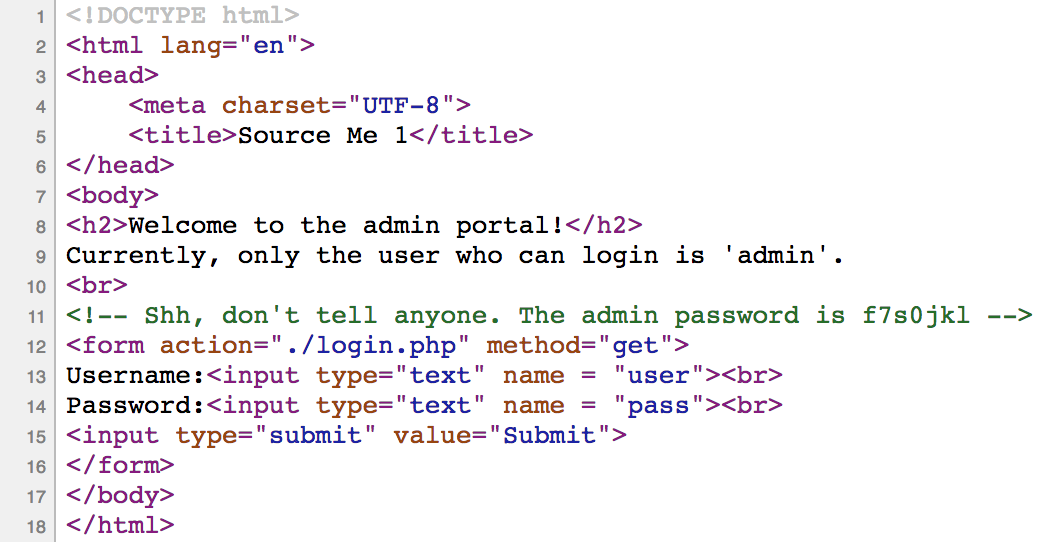
\includegraphics[width=10cm]{flag_page_source}
\caption{Flaga \textbf{f7s0jkl} ukryta w źródle strony internetowej}
\label{fig:flag_page_source}
\end{figure}

W mojej pracy będę prezentował jednak grę opartą
wyłącznie o Reverse Engineering (ang. Inżynieria Wsteczna).
Inżynieria wsteczna oprogramowania może odbywać się na różne sposoby.
Może to być przykładowo wykorzystanie tzw. snifferów do analizy protokołów
komunikacji aplikacji internetowej. W naszym wypadku będzie ona jednak
zazwyczaj oznaczała proces analizy programu, aby zrozumieć co robi
oraz w jaki sposób. Zadania, które przedstawie można by też podpiąć do kategorii
eksploitacji binarnej (ang. Binary Exploitation), która w pewny sposób pokrywa
się z zagadnieniami Reverse Engineeringu. Jest to mianowicie proces
wykorzystywania niedoskonałości programów w celu zmuszenia ich do zrobienia
czegoś, czego w normalnej sytuacji nie powinny robić. Te dwie kategorie pokrywają
się ze sobą, ponieważ zazwyczaj nie jest możliwe rozwiązanie zadania z kategorii
eksploitacji binarnej, bez wykorzystania do tego inżynierii wstecznej.

%\emph{Charakterystyka problemu, motywacja projektu (w tym przegląd
%  istniejących rozwiązań prowadząca do uzasadnienia celu prac),
%  wizja produktu i analiza zagrożeń.}

\section{\SectionTitleScope}
\label{sec:zakres-funkcjonalnosci}
%\emph{Kontekst użytkowania produktu (aktorzy, współpracujące systemy)
%  oraz specyfikacja wymagań funkcjonalnych i niefunkcjonalnych.}

\section{\SectionTitleRealizationAspects}
\label{sec:wybrane-aspekty-realizacji}
% \emph{Przyjęte założenia, struktura i zasada działania systemu,
%   wykorzystane rozwiązania technologiczne wraz z uzasadnieniem
%   ich wyboru, istotne mechanizmy i zastosowane algorytmy.}

\section{\SectionTitleWorkOrganization}
\label{sec:organizacja-pracy}
% \emph{Struktura zespołu (role poszczególnych osób), krótki opis i
%   uzasadnienie przyjętej metodyki i/lub kolejności prac, planowane i
%   zrealizowane etapy prac ze wskazaniem udziału poszczególnych
%   członków zespołu, wykorzystane praktyki i narzędzia w zarządzaniu
%   projektem.}

\section{\SectionTitleResults}
\label{sec:wyniki-projektu}
% \emph{Wskazanie wyników projektu (co konkretnie udało się uzyskać:
%   oprogramowanie, dokumentacja, raporty z testów/wdrożenia, itd.), prezentacja wyników
%   i ocena ich użyteczności (jak zostało to zweryfikowane --- np.\ wnioski
%   klienta/użytkownika, zrealizowane testy wydajnościowe, itd.),
%   istniejące ograniczenia i propozycje dalszych prac.}

% o ile to możliwe proszę używać odwołań \cite w konkretnych miejscach a nie \nocite

% \nocite{artykul2011,ksiazka2011,narzedzie2011,projekt2011}

% \bibliography{bibliography}

\end{document}
